\documentclass{beamer} \setbeamertemplate{navigation symbols}{}

\usepackage{amsmath}

 

\title[Collective SRL with ML]{Collective Semantic Role Labelling with
  Markov Logic} \author[Riedel and Meza]{Sebastian Riedel \qquad Ivan
  Meza-Ruiz}
\institute[ICCS, UoE]{Institute for Communicating and Collaborative Systems\\
  School of Informatics\\
  University of Edinburgh\\
  {\tt\{S.R.Riedel,I.V.Meza-Ruiz\}@sms.ed.ac.uk} } \date{August 16th,
  2008}

\usetheme{Madrid}

\begin{document}
\begin{frame}
  \titlepage
\end{frame}

\begin{frame}
  \frametitle{ SRL Intuitions: Local}
  \begin{center}
    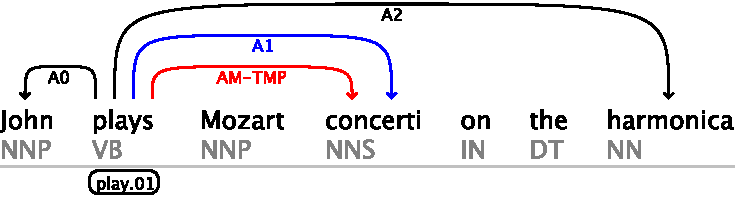
\includegraphics[scale=.70]{example-3}
  \end{center}

  \begin{itemize}
  \item Semantic role label of a token correlates with its POS tag
  \end{itemize}
\end{frame}


\begin{frame}
  \frametitle{ SRL Intuitions: Global}
  \begin{center}
    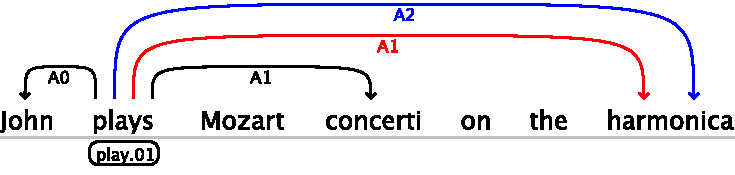
\includegraphics[scale=.70]{example-2}
  \end{center}
   
  \begin{itemize}
  \item A predicate can have at most one semantic argument of each
    type.
  \end{itemize}
\end{frame}


\begin{frame}
  \frametitle{ SRL Intuitions: Global And Soft}
  \begin{center}
    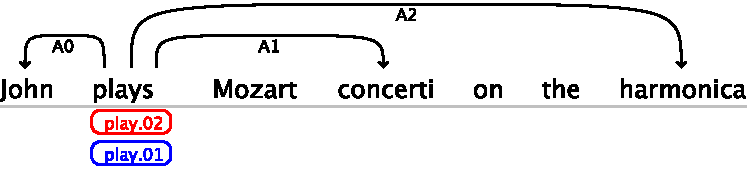
\includegraphics[scale=.70]{example-1}
  \end{center}

  \begin{itemize}
  \item Sense of a verb correlates with the roles of its
    arguments/modifiers.
  \end{itemize}
\end{frame}


\begin{frame}
  \frametitle{Capturing intuitions}

  %SR: I put some pauses in here. I feel that this slide is crucial and sets the stage for everything else. So take your time with this one
    
  How do we capture such intuitions?

  \pause

  \begin{itemize}
  \item Local: off-the-shelf classifier, easy to do, (not much Machine
    Learning expertise necessary) \pause
  %SR: we need some cites here I think 
  \item Global: pipeline, reranking, ILP, approximate heuristic
    search, harder to engineer, (more Machine Learning expertise
    necessary.)
  \end{itemize}

  \pause
     
  Markov Logic (generally: Statistical relational learning):
  \begin{itemize}

  \item capture local and global intuition using weighted first order
    formula
  \item run off-the-shelf training and inference software
  \end{itemize}



    
\end{frame}

\begin{frame}
  \frametitle{Overview}
  \tableofcontents
\end{frame}

\section{Markov Logic}

\begin{frame}
  \frametitle{Markov Logic [Richardson \& Pedro (2005)]}

  What?
  \begin{itemize}
  \item Combines of FOL and Markov Networks
  \item Defines a log-linear distribution over possible worlds
  \item Uses weighted FOL formulae
  \end{itemize}
  Why?
  \begin{itemize}
  \item Decoupling: fosters independent progress in Machine Learning
    and application domains
  \item Induction: automatically induce new rules
  \item Efficiency: first order representation can be exploited in
    inference and learning
  \end{itemize}


\end{frame}

\begin{frame}
  \frametitle{Vocabulary}
  The vocabulary consists of:
  \begin{itemize}
  \item \textbf{Constants} represent objects of the domain (e.g., Haag,
    VB, 1, 2, 3, \ldots)
  \item \textbf{Predicates} represent relations over the objects
  \end{itemize}
  \bigskip There are two types of predicates: observable and
  hidden. \\Some of the observable predicates are:
  \begin{itemize}
  \item \textbf{word/2}, \emph{word(1,Haag)}
  \item \textbf{pos/2}, \emph{pos(1,NNP)}
  \item \textbf{path/3}, \emph{path(2,1,$\uparrow\uparrow\downarrow$)}
  \end{itemize}
    
\end{frame}

\begin{frame}
  \frametitle{Hidden predicates}
  \begin{figure}
    \begin{center}
      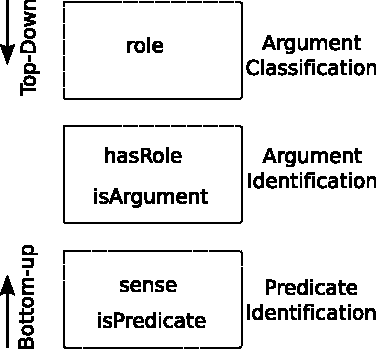
\includegraphics[scale=.70]{TaskArchitecture}
    \end{center}
    \caption{Hidden predicates}
    \label{fig:task}
  \end{figure}

  Input : \[\{word(1,Mr.),word(2,Haag), word(3,plays),
  word(4,elianti), \ldots \}\] Output : \[\{isPredicate(3),
  sense(3,02), isArg(2), hasRole(3,2), role(3,2,A0), \ldots \}\]

\end{frame}

\section{Modelling}


% do we need this slide?
% \begin{frame}
%   \frametitle{Formulae}
%   We use formulae to capture intuitions about the problem

%   \begin{itemize}
%   \item Local formulae \bigskip
%   \item Global formulae
%   \end{itemize}
% \end{frame}

\begin{frame}
  \frametitle{Formulae: Local}
    
  \begin{center}
    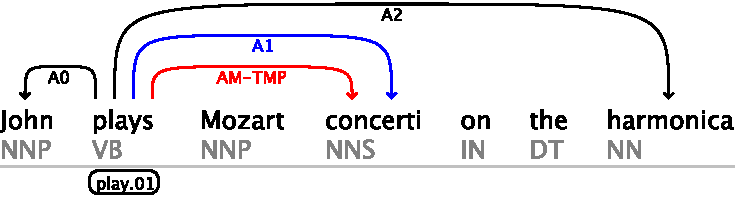
\includegraphics[scale=.70]{example-3}
  \end{center}

  \begin{itemize}
  \item Semantic role label of a token correlates with its POS tag
  \end{itemize}

  \[ppos(p,+p_p) \wedge ppos(a,+p_a) \Rightarrow role(p,a,+r)\]

\end{frame}


\begin{frame}
  \frametitle{Formulae: Global}
  \begin{center}
    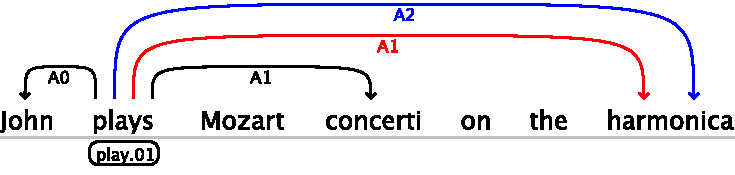
\includegraphics[scale=.70]{example-2}
  \end{center}

  \begin{itemize}
  \item A predicate can have at most one semantic argument of each
    type.
  \end{itemize}

 \begin{eqnarray*}
   &role\left(p,a_{1},r\right)\wedge \neg mod\left(r\right)\wedge a_{1}\neq a_{2}  \Rightarrow\\
   & \neg role\left(p,a_{2},r\right)
 \end{eqnarray*}


\end{frame}


\begin{frame}
  \frametitle{Formulae: Global and Soft}
  \begin{center}
    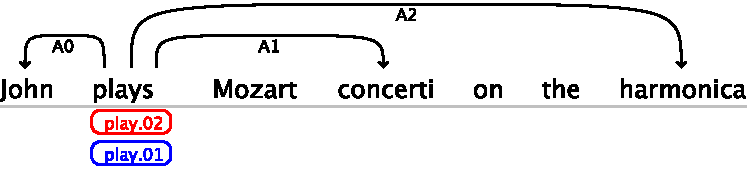
\includegraphics[scale=.70]{example-1}
  \end{center}

  \begin{itemize}
  \item Sense of a verb correlates with the roles of its
    arguments/modifiers.
  \end{itemize}

  \begin{eqnarray*}
    & lemma(p,+l) \wedge ppos(a,+s)  \\
    & \wedge hasRole(p,a)  \Rightarrow sense(p,+f) 
  \end{eqnarray*}

\end{frame}


\begin{frame}
  \frametitle{Formulae: Summary}

  Implemented: 
  \begin{itemize}
  \item Local formulae [Xue \& Palmer (2004)]
  \item Global formulae for one predicate
  \item Global formulae for two different predicates (Structural formulae)\\
      \begin{eqnarray*} & & isPredicate/1 \leftrightarrow sense/2 \\ 
         & & isPredicate/1 \leftrightarrow isArgument/1 \\
         & & isArgument/1 \leftrightarrow hasRole/2  \\
         & & hasRole/2 \leftrightarrow role/3 \\
      \end{eqnarray*}
  \end{itemize}
\end{frame}


\begin{frame}
  \frametitle{Markov Logic Network}
  Collect weighted formulae into a \textbf{Markov Logic Network} (MLN).

  An MLN defines a Markov Network where:
  \begin{itemize}
  \item There is a binary node for each ground atom (e.g.,
    \emph{role(2,1,A1)}.)
  \item There is a factor for each assignment of the free variable of
    each formulae.
  \end{itemize}

  \begin{center}
    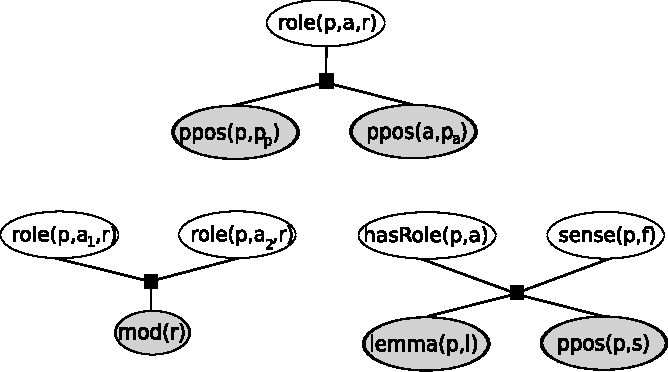
\includegraphics[scale=.55]{factor_graphs}
  \end{center}

  % SR: show simple small ground network

  % \begin{eqnarray*}
  %   \prob\left(\y\right)=\frac{1}{Z}\exp\left(
  %     \sum_{\left(\phi,w\right)\in M} w \sum_{\boldc\in
  %       C^{n_{\phi}}}f_{\boldc}^{\phi}\left(\y\right) \right)
  % \end{eqnarray*}

\end{frame}

\section{Experiments}
\begin{frame}
  \frametitle{Experiments}

  \begin{itemize}
  \item Full model: includes all the rules we came up with.
    % SR: do you think this explanation of Bottom-up vs top-down rules
    % is faithful to what happens (I had problems seeing it that way)
    % -- Should we maybe add one more slide for this (maybe discarding
    % the "Modelling" slide)?
  \item Bottom-Up model: discard top-down rules, it resembles a
    pipeline where candidates are picked by latter module.
  \item Top-down model: discard bottom-up rules, it resembles a
    pipeline where candidates are picked by earlier module.
  \item Isolated: discard bottom-up and top-down rules.
  \item Structural: discard the soft global rules.
  \end{itemize}
\end{frame}

\begin{frame}
  \frametitle{Results}

  \begin{table}
    \begin{center}
      \small
      \begin{tabular}{|l|l|l|c|c|}\hline
        Model                & WSJ                & Brown              & Train & Test\\
        &                    &                    & Time & Time\\\hline\hline
        Full         & $75.72\%$          & $\mathbf{65.38}\%$ & 25h & 24m\\\hline
        Up           & $\mathbf{76.96\%}$ & $63.86\%$          & 11h & 14m\\\hline
        Down         & $73.48\%$          & $59.34\%$          & 22h & 23m\\\hline
        Isolated     & $60.49\%$          & $48.12\%$          & 11h & 14m\\\hline
        Structural   & $74.93\%$          & $64.23\%$          & 22h & 33m\\\hline   
      \end{tabular}
      \caption{F-scores for different models.}
      \label{tbl:results}
      \normalsize
    \end{center}
  \end{table}
\end{frame}

\section{Conclusion}
\begin{frame}
  \frametitle{Conclusions}

  \begin{itemize}
  \item This network achieves the second best semantic F- scores in
    the Open Track of the CoNLL shared task for only SRL.  \bigskip
  \item The bottom-up model outperforms the full model on WSJ.
  \item ML: minimal engineering efforts + state-of-the-art results.
  \end{itemize}
\end{frame}

\begin{frame}
  \frametitle{Pointers}

  \begin{itemize}
  \item Implementation of ML:\\
    \texttt{http://thebeast.googlecode.com/} \bigskip
  \item Models and scripts:\\
    \texttt{http://thebeast.googlecode.com/svn/mlns/conll08/}
  \end{itemize}
\end{frame}



\end{document}
